\documentclass[fleqn, a4paper]{report}

%% Language and font and usefull packages
\usepackage[english]{babel}
\usepackage[utf8x]{inputenc}
\usepackage{booktabs}
\usepackage{tabu}
\usepackage[T1]{fontenc}
\usepackage{bm}
\usepackage{dsfont}
\usepackage{setspace}
\usepackage{amsmath}
\usepackage{graphicx}
\usepackage{fontawesome}
\usepackage{titlepic}
\usepackage{fixltx2e}
\usepackage{booktabs} % For prettier tables
\usepackage[colorinlistoftodos]{todonotes}
\usepackage[colorlinks=true, allcolors=blue]{hyperref}

\usepackage[a4paper,top=2cm,bottom=2cm,left=1cm,right=1cm,marginparwidth=1.75cm]{geometry}

%\graphicspath{ {./images} }
\title{Assignment 2 - Simulation Experiment}
\author{
Theodoros Ladas - s2124289 
\footnote{University of Edinburgh s2124289@ed.ac.uk}
}
\titlepic{
\includegraphics[width=12.528cm,height=3cm]{./images/edinburgh.png}} 
\date{\parbox{\linewidth}{\centering%
  February 4, 2021\endgraf\bigskip
  Coordinator: Miguel de Carvalho\endgraf\medskip
  Dept.\ of Mathematics \endgraf
  University of Edinburgh}}


\onehalfspacing
\begin{document}
\maketitle

\section*{1. Experiment}

The goal of this experiment is to compare the kernel density estimation (from now on KDE) method, with a Gaussian kernel with some other method, in order to see under which circumstances should each one be used. The data generation process, the comparison, the final error score, and the diagrams are produced using the $R$ language.
\\
\text{Let} $X_1,X_2,...,X_n \overset{\text{iid}}{\sim} f$. The KDE of $f$ is defined as
\begin{align*}
\hat{f}(x) = \frac{1}{nh}\sum_{i=1}^n \frac{K(x-X_i)}{h}
\end{align*}
where $K_h()$ is a density (kernel) and $h>0$ is a parameter controlling the smoothness of the estimate called \textit{bandwidth}.
The experiment is divided into two main stages. First, we will compare the histogram and the KDE, to build some understanding on some well-defined cases, and then we will continue with a Monte Carlo experiment, where we will compare numerically the KDE to the true distribution that we are trying to approximate, using the Integrated Squared Error metric, which is defined as,
\begin{align*}
\textbf{ISE} = \int_X \{\hat{f}(x) - f(x)\}dx
\end{align*}
where $f(x)$ is the true distribution of the data. The histogram can be thought of as a continuous extension of the bar plot where the range of the observations is divided into $k$ nonoverlapping and successive bins $B_1, . . . , B_k$. We then count the number of samples
falling into each bin $B_j$: $n_j = \sum_{i=1}^n \mathds{1}_{B_j}(x_i)$. We can normalize the $n_j$ by $n$ to show the relative frequencies. The bins are often chosen to have equal bin width $h$ \cite{arno_data_2020}.

\subsection*{1.1. Data generating processes}
For the first stage of the experiment, the data have been generated from three different distribution, with a split for small and big datasets. Small datasets have an $n=200$, while big datasets are $n=1e6$ and the true distributions of the data are $f_1(x) = N(x; \mu=0, \sigma=1)$, $f_2(x) = \text{Gamma}(x; \text{shape}=5, \text{rate}=1)$, 
$f_3(x) = \text{M}f_1(x) + (1-\text{M})f_2(x)$, where $\text{M} \in [0,1]$ is a hyper-parameter, that controls the mixing of the two distributions. For the purposes of the experiment, we choose a hyper-parameter of $\text{M} = 0.5$, in order to have a 50\%-50\% split between the Normal and the Gamma distributions. 

For the second stage of the experiment, the same $f_1(x), f_2(x), f_3(x)$ where chosen, but the number of samples $n$ was allowed to vary from $n=100$ to $n=2000$ with a step of $50$. The numerical results of the MISE are presented on a table for $n=250,500,1000$, but there is also a graph that reported the three distributions with the MISE produced in every step, to check whether the error seems to converge or not on a given number. The simulation was structured in the following manner. First we create for each distribution $R=1000$ rows of samples of each $n$ samples of the $f_1(x), f_2(x), f_3(x)$ distributions. Then we average by column the given samples using the mean of the column. Thus we have a vector of size $n$ generated from $1000$ samples. Then we estimate the distribution with KDE and measure the ISE from the true distributions. 

Before we move on to the results of each stage of the experiment, we need to also be completely transparent about the process of setting the hyper-parameters of the model. The most important hyper-parameter for the histogram is the number of bins used, while for KDE is the \textit{bandwidth} $h$. The bins were chosen as a fixed number and more specifically, for the small dataset the bins are $20$, while for the large datasets are $30$. After manually checking various examples these were the final numbers. For the \textit{bandwidth}, we tried to create a function to minimize the Euclidean distance of the KDE and the real distribution. This is \textbf{not} a valid way of setting the hyper-parameter in a real-life application since we won't have access to the true distribution, however for the purposes of comparing the best possible outcome of the KDE \textit{versus} the best possible outcome of the histogram this can be thought of as a fair comparison. However in the end the output of the function was clearly not correct and instead we used the default function in $R$ to set the bandwidth. This is left in the code for further improvement on the experiment. 
\subsection*{1.2. KDE vs Histogram}
On \textit{Figure 1} we can see the six different cases. 
\begin{figure}[!ht]
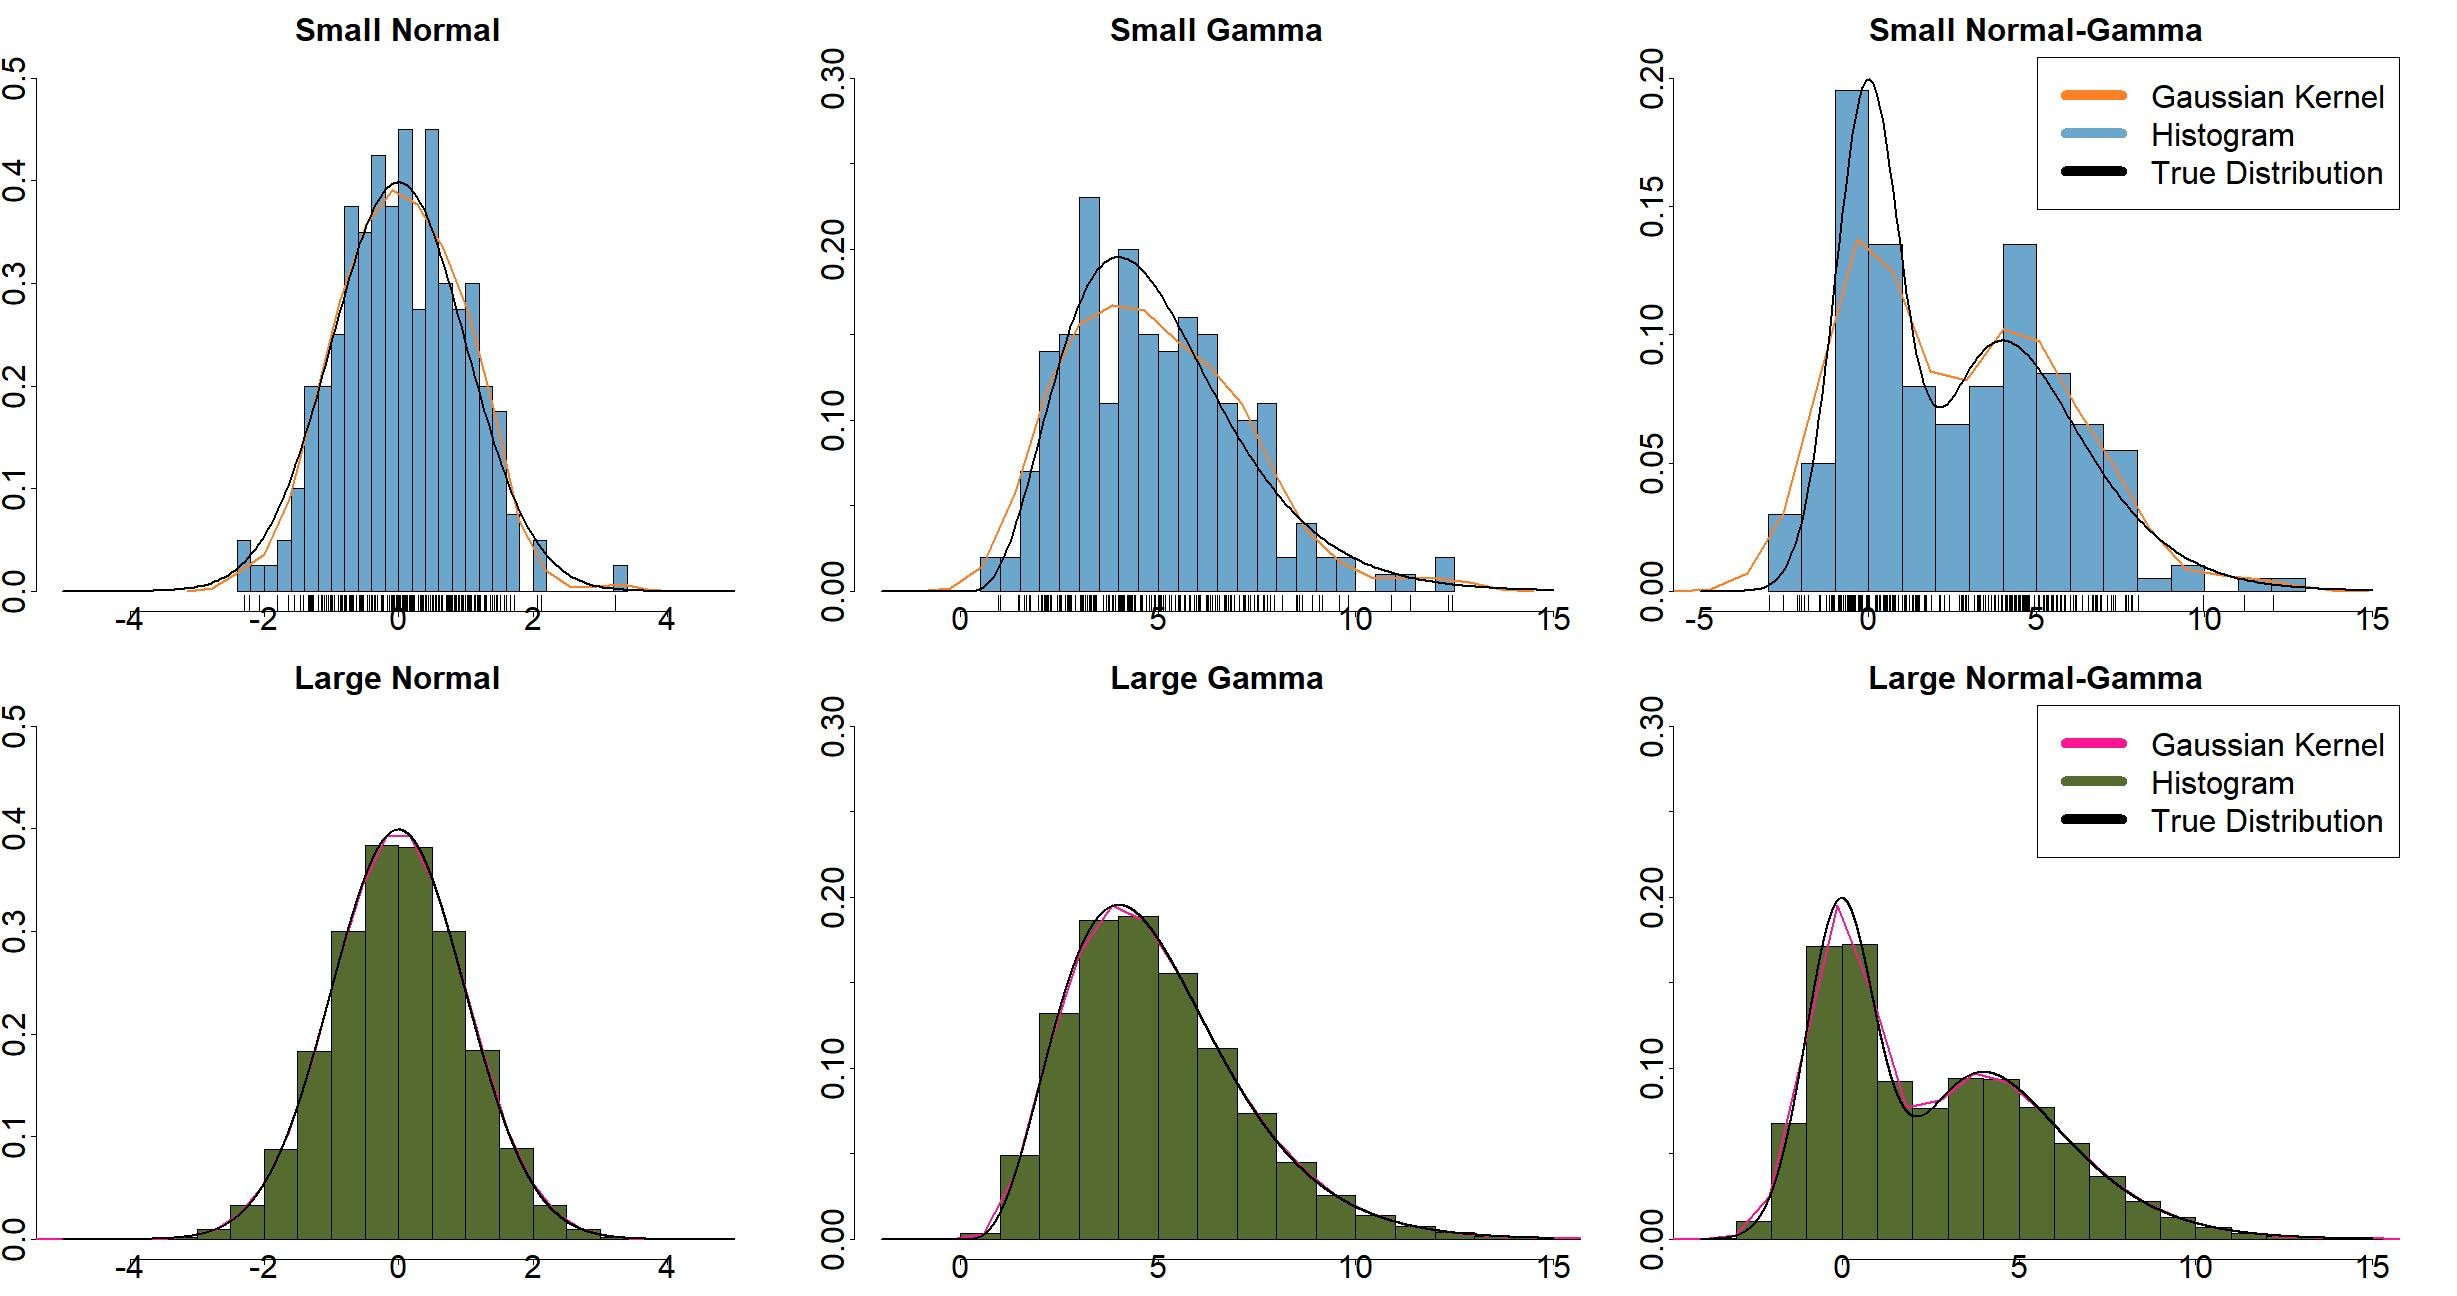
\includegraphics[width=0.82\textwidth]{./images/hist_vs_GKDE.jpg}
\textsubscript{\textit{Figure 1}}
\label{tab:fig_1}
\end{figure}
On the first line, we see the results for the small datasets and the second one, for the large datasets. The black lines represent the true densities, while the colored lines represent the KDE. With this diagram, the reason for the split into a small and large dataset is immediately apparent. As $n \rightarrow \infty$, both estimation methods become \textit{good} approximation of the true distributions. In this case, where we use the \textit{Gaussian} kernel, the KDE seems to be pretty capable of producing a Normal, a Gamma as well as a mixture of Normal Gamma distributions since it follows the true PDF. 

On the other hand, when we shift our attention to the first row, we can see two things. First of all, the histogram is overestimating the probability mass of some of the bins, while underestimating the mass on others. The default setting for the \textit{bandwidth} of the KDE is doing a much better job at estimating the small Normal distribution than the histogram. However, we can easily notice that in the other cases, except for the Normal distribution, the KDE is not that accurate. The fact that the number of samples is small, seems to have a lot of impact on both methods and neither is estimating accurately the true distribution. The most obvious example is the second one, where the true distribution is the Gamma. In this case, neither the histogram nor the KDE mean values are close to the true distribution mean which is $5$. A very important point that has to be highlighted, is that the choice of the bandwidth is extremely important. In our experiments, when the bandwidth was chosen to be a fixed number and not by optimizing some cost function, the KDE would either be very flat and give a lot of mass to the tails of the distribution, or extremely \textit{sensitive}, which is represented by a very jagged multimodal PDF. This process seems to resemble the process of over/under fitting in Machine learning, where some parameter of the model, here the bandwidth which represents the complexity/detail at which we are trying to estimate the true distribution, needs to be carefully chosen for the model to be able to generalize well \cite{murray_machine_2020}.

Finally, a very important comment about KDE needs to be made at this point that is not very apparent from the diagrams. In the case of the Gamma model, we know that the support of the Gamma function is $[0, +\infty)$. However, we can see that the KDE puts some mass on negative values as well. The histogram is much better in that sense since it doesn't allocate mass to impossible values of the distribution, that are lower than the left boundary of the distribution. This problem can be bypassed by mirroring the data. Then we sum the original and mirrored KDEs and finally set the probability to zero before the lower boundary \cite{kang2018kernel}. This shows once again the importance of thinking very carefully about the specific problem we are trying to solve.


\section*{2. Monte Carlo Simulation}
Now that the first section is over, we can continue our experimentation and quantify the results with an MCMC simulation. As described above, we will produce the Mean Integrated Squared Error (MISE) of the KDE of our generated sample from each distribution and the true distribution for various sample sizes. The point of this experiment is to quantify the distance between the estimated and true density and to check, whether for a given \textit{bandwidth} $h$, the distance converges to some minimum. On \textit{Table 1} the results for $n=250,500,1000$ are presented for the same three distributions we were using above (Normal, Gamma, and Normal-Gamma mixture). 

\begin{table}[]
\centering
\begin{tabular}{|l|lll|}
\hline
n & Normal & Gamma & Mixture \\ \hline
250 & 8.612 & 4.092 & 0.092 \\
500 & 8.013 & 3.994 & 0.101 \\
1000 & 8.095 & 3.879 & 0.117 \\ \hline
\end{tabular}
\caption{MISE}
\label{tab:table_1}
\end{table}

Here we have some expected and some not so, results. First of all, we see that for the normal case, the results for the small and large sample sizes are similar. That means that the approximation is independent of these sample sizes. Of course, there is some variability (from $8.61$ to $8.09$). This is expected, as, from the above example, we know that the KDE with a Gaussian kernel, is a very good approximation of the true Normal distribution, both for small and large sample values. We see almost the same for the Gamma case. Lastly, the most important result from this table is the not expected one. On the mixture model, we see a small but apparent upward trend in the error. From our Histogram vs KDE experiment, we should expect the opposite. This motivated us to produce the following figure. 

\begin{figure}[!h]
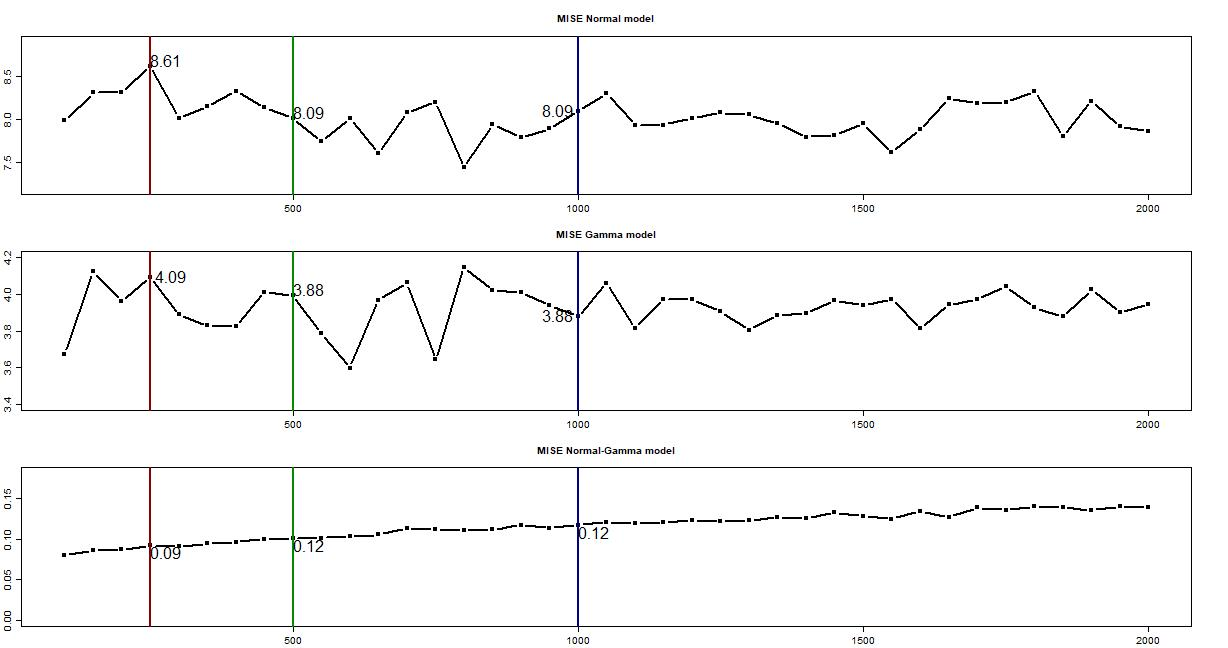
\includegraphics[width=0.82\textwidth]{./images/MISE error.jpg}
\textsubscript{\textit{Figure 2}}
\label{tab:fig_2}
\end{figure}

In \textit{Figure 2} we can see the same error as in the above table, but sampled for many more $n$ from $n=100$ up to $n=2000$. While the first and the same diagram show no visible trend, the third one does. At this point, the root cause analysis for this phenomenon stopped, and this remains the most important caveat in the whole model. We saw on the first part that the KDE for the mixture model and $n=1e6$ was estimating the true density well. However, the MCMC experiment was computationally expensive to run up to such large numbers to quantify that MISE. This is future work that needs to be done to fully justify the results. 

\section*{3. Conclusion}
We have seen that both KDE and the histogram method, are a pretty good approximation of a true distribution when the number of samples is sufficiently large. For small samples, the histogram fails to capture the true PDF, but has a major advantage over the KDE, that it's impossible for the histogram to put mass on impossible values in the case of a bounded domain. Lastly, further work needs to be conducted to quantify the MISE of the KDE and the true PDF, for the Normal-Gamma mixture model as it seems that $n=2000$ is not sufficiently large.

The code for the above experiment can be found on my \href{https://github.com/TedOiler/SRS/tree/master/Assignment_2}{\faGithub} page. This repository is a private one, that I will make public after the assignment deadline and turn private again when the assignment is graded.

\bibliographystyle{plain}
\bibliography{assignment_2_references.bib}

\end{document}
























